\documentclass[12pt]{memoir}

\def\nsemestre {II}
\def\nterm {Fall}
\def\nyear {2022}
\def\nprofesor {Maria Gillespie}
\def\nsigla {MATH501}
\def\nsiglahead {Combinatorics}
\def\nextra {HW12}
\def\nlang {ENG}
\input{../../headerVarillyDiff}

\begin{document}
\iffalse
\begin{Ej}[Exercise 1]
    Among a family of 20 people, 9 of them like chocolate ice cream, 7 of them like vanilla ice cream, and 2 like both chocolate and vanilla. How many don't like either flavor of ice cream? Explain how the Inclusion-Exclusion principle applies here.
 \end{Ej}

\begin{ptcbr}
   Call $F$ the set of family members, $C$ the set of people who like chocolate ice cream and $V$ the ones who like vanilla. The set $F$ can be partitioned as 
   $$F=(C\cup V)\cupdot (C\cup V)^c$$
   where $(C\cup V)^c$ is the set of family members who dislike both flavors. This is the set we are looking for.\par 
   By Inclusion-Exclusion applied to the two sets $C,V$ we have 
   $$|C\cup V|-|C|-|V|+|C\cap V|=0\To |C\cup V|=9+7-2=14.$$
   As the whole family has 20 members and 14 of them like either flavor of ice cream, then 6 of them dislike both flavors.\par 
   We must use the Inclusion-Exclusion formula to find the size of the union, by summing only $|C|$ and $|V|$ we would be overcounting the the ones who like both flavors.
\end{ptcbr}
\fi
\begin{Ej}[Exercise 2]
    Let $P$ be a poset in which every interval $[x, y]$ is finite. Show that, in the incidence algebra $\mathscr{I}(P)$:
    \vspace*{-0.4em}
    \begin{enumerate}[i)]
        \itemsep=-0.4em
        \item $f$ is invertible if and only if $\forall x(f(x,x)\neq 0)$.
        \item $fg=\dl\iff gf=\dl$, this is, inverses are two sided.
        \item If $f$ is invertible then $f^{-1}$ is unique.
    \end{enumerate}
\end{Ej}

Really quickly, recall that the incidence algebra is the set of \emph{interval functions} from $P$ to $\bC$. In other words, we can describe $\mathscr{I}(P)$ as 
$$\mathscr{I}(P)=\set{f:P^2\to\bC:\ x>y\To f(x,y)=0}.$$

\begin{ptcbr}
    \begin{enumerate}[i)]
        \itemsep=-0.4em
        \item Suppose $f$ is invertible with $fg=\dl$. If $x\in P$:
        $$(f\.g)(x,x)=f(x,x)g(x,x)=\dl(x,x)=1.$$
        This means that, as complex numbers, $f(x,x)g(x,x)=1$ thus none can be zero and $f(x,x)=\frac{1}{g(x,x)}$.\par 
        On the other hand, suppose $f(x,x)\neq 0$. We will construct an inverse for $f$ inductively using the fact the every interval is finite.\par
        Our base case is $|[x,y]|=1$, then $x=y$ and $g(x,x)=\frac{1}{f(x,x)}$. Suppose that we have an interval $[x,y]$ of length $n$ and for intervals of length less than $n$ $g(x,y)$ is the inverse of $f(x,y)$. So 
        \begin{align*}
            \dl(x,y)=(fg)(x,y)\iff &0=\sum_{x\leq z\leq y}f(x,z)g(z,y)\\
            \iff &0=f(x,x)g(x,y)+\sum_{x< z\leq y}f(x,z)g(z,y)\\
            \iff &-f(x,x)g(x,y)=\sum_{x< z\leq y}f(x,z)g(z,y)\\
            \iff &g(x,y)=\frac{-1}{f(x,x)}\sum_{x< z\leq y}f(x,z)g(z,y)
        \end{align*}
        Thus it holds that when $f(x,x)\neq 0$, we can solve the previous equation to obtain an expression for the inverse of $f$. By induction, it follows that $f$ is invertible. 
        \item First notice that the process we did in the last item is valid even if we replace \emph{invertible} with \emph{right-invertible}. The same process can be done in the same way to obtain a \emph{left inverse} for $f$ such that $hf=\dl$. This means that $hf=fg\To h=g$.
        %\item If $g,h$ are two inverses for $f$, then $fg=\dl=fh\To g=h$ once again. 
        \iffalse\par 
        Even if it's not stated, I assume that the objective of this exercise is not to mention a fact about the algebra itself but instead to verify that the formula is valid. So let us proceed by taking $g$, $f$'s right inverse as in the last item and showing it also is a left inverse. 
        \begin{align*}
            (gf)(x,y)&=\sum_{x\leq z\leq y}g(x,z)f(z,y)\\
            &=\sum_{x\leq z\leq y}\left(\frac{-1}{f(x,x)}\sum_{x< t\leq z}f(x,t)g(t,z)\right)f(z,y)\\
            &=\sum_{x\leq z\leq y}\left(\frac{-1}{f(x,x)}\left(\sum_{x< t< z}f(x,t)g(t,z)+f(x,z)g(z,z)\right)\right)f(z,y)\\
        \end{align*}
        \fi
    \end{enumerate}
\end{ptcbr}

\begin{Ej}[Exercise 3, Sagan 5.27]
    Consider Young's lattice $Y$ of all integer partitions ordered by containment of Young diagrams. Given $\la$, consider the interval $P_\la=[(1),\la]$ as a subposet of $Y$. Recall $|\la|=n$ when $\la\vdash n$.
    \vspace*{-0.4em}
    \begin{enumerate}[i)]
        \itemsep=-0.4em
        \item Compute $\mu(P_\la)$ for $1\leq|\la|\leq 3$. 
        \item Show that $\mu(P_\la)=0$ for $|\la|\geq 4$.
    \end{enumerate}
\end{Ej}

\begin{ptcbr}
    \begin{enumerate}[i)]
        \itemsep=-0.4em
        \item We will draw Young's lattice and add the values of the Möbius function to each of the elements right next to them:
        \begin{center}
            

\tikzset{every picture/.style={line width=0.75pt}} %set default line width to 0.75pt        

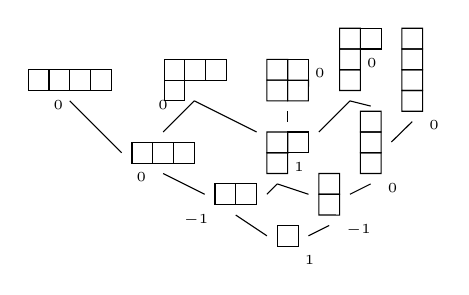
\begin{tikzpicture}[x=0.75pt,y=0.75pt,yscale=-1,xscale=1]
%uncomment if require: \path (0,300); %set diagram left start at 0, and has height of 300

%Shape: Square [id:dp3373686653034773] 
\draw   (200,280) -- (210,280) -- (210,290) -- (200,290) -- cycle ;
%Shape: Square [id:dp2924781376289838] 
\draw   (170,260) -- (180,260) -- (180,270) -- (170,270) -- cycle ;
%Shape: Square [id:dp8666374063990736] 
\draw   (180,260) -- (190,260) -- (190,270) -- (180,270) -- cycle ;
%Shape: Square [id:dp7107668927495867] 
\draw   (130,240) -- (140,240) -- (140,250) -- (130,250) -- cycle ;
%Shape: Square [id:dp9372183522191804] 
\draw   (140,240) -- (150,240) -- (150,250) -- (140,250) -- cycle ;
%Shape: Square [id:dp7414297981189042] 
\draw   (150,240) -- (160,240) -- (160,250) -- (150,250) -- cycle ;
%Shape: Square [id:dp7984772395054516] 
\draw   (80,205) -- (90,205) -- (90,215) -- (80,215) -- cycle ;
%Shape: Square [id:dp3323819129604224] 
\draw   (90,205) -- (100,205) -- (100,215) -- (90,215) -- cycle ;
%Shape: Square [id:dp6917898843068055] 
\draw   (100,205) -- (110,205) -- (110,215) -- (100,215) -- cycle ;
%Shape: Square [id:dp6324017168656659] 
\draw   (110,205) -- (120,205) -- (120,215) -- (110,215) -- cycle ;
%Shape: Square [id:dp901247195887662] 
\draw   (270.03,185.01) -- (270.02,195.01) -- (260.02,195) -- (260.03,185) -- cycle ;
%Shape: Square [id:dp6975974541523413] 
\draw   (270.02,195.01) -- (270.01,205.01) -- (260.01,205) -- (260.02,195) -- cycle ;
%Shape: Square [id:dp7332951946092128] 
\draw   (270.01,205.01) -- (270.01,215.01) -- (260.01,215) -- (260.01,205) -- cycle ;
%Shape: Square [id:dp7998208729214848] 
\draw   (270.01,215.01) -- (270,225.01) -- (260,225) -- (260.01,215) -- cycle ;
%Shape: Square [id:dp25209857454270757] 
\draw   (250.02,225.01) -- (250.01,235.01) -- (240.01,235) -- (240.02,225) -- cycle ;
%Shape: Square [id:dp4584871677228517] 
\draw   (250.01,235.01) -- (250.01,245.01) -- (240.01,245) -- (240.01,235) -- cycle ;
%Shape: Square [id:dp9392012086346246] 
\draw   (250.01,245.01) -- (250,255.01) -- (240,255) -- (240.01,245) -- cycle ;
%Shape: Square [id:dp4815673839754695] 
\draw   (230.01,255.01) -- (230.01,265.01) -- (220.01,265) -- (220.01,255) -- cycle ;
%Shape: Square [id:dp16720372206692558] 
\draw   (230.01,265.01) -- (230,275.01) -- (220,275) -- (220.01,265) -- cycle ;
%Shape: Square [id:dp8639269656814101] 
\draw   (205.01,235.01) -- (205.01,245.01) -- (195.01,245) -- (195.01,235) -- cycle ;
%Shape: Square [id:dp013642674735359517] 
\draw   (205.01,245.01) -- (205,255.01) -- (195,255) -- (195.01,245) -- cycle ;
%Shape: Square [id:dp7243712982718384] 
\draw   (205.01,235.01) -- (215.01,235.01) -- (215.01,245.01) -- (205.01,245.01) -- cycle ;
%Shape: Square [id:dp48859881467651944] 
\draw   (205.01,200.01) -- (205.01,210.01) -- (195.01,210) -- (195.01,200) -- cycle ;
%Shape: Square [id:dp2702085858580814] 
\draw   (205.01,210.01) -- (205,220.01) -- (195,220) -- (195.01,210) -- cycle ;
%Shape: Square [id:dp0661071729061169] 
\draw   (205.01,200.01) -- (215.01,200.01) -- (215.01,210.01) -- (205.01,210.01) -- cycle ;
%Shape: Square [id:dp39762328755409326] 
\draw   (240.02,185.01) -- (240.01,195.01) -- (230.01,195) -- (230.02,185) -- cycle ;
%Shape: Square [id:dp534170828730052] 
\draw   (240.01,195.01) -- (240.01,205.01) -- (230.01,205) -- (230.01,195) -- cycle ;
%Shape: Square [id:dp7815852339268066] 
\draw   (240.01,205.01) -- (240,215.01) -- (230,215) -- (230.01,205) -- cycle ;
%Shape: Square [id:dp15506838920862465] 
\draw   (240.02,185.01) -- (250.02,185.01) -- (250.02,195.01) -- (240.02,195.01) -- cycle ;
%Shape: Square [id:dp6838769532238735] 
\draw   (145.5,200) -- (155.5,200) -- (155.5,210) -- (145.5,210) -- cycle ;
%Shape: Square [id:dp011720447522689525] 
\draw   (155.5,200) -- (165.5,200) -- (165.5,210) -- (155.5,210) -- cycle ;
%Shape: Square [id:dp9276531047224357] 
\draw   (165.5,200) -- (175.5,200) -- (175.5,210) -- (165.5,210) -- cycle ;
%Shape: Square [id:dp49948983980702866] 
\draw   (145.5,210) -- (155.5,210) -- (155.5,220) -- (145.5,220) -- cycle ;
%Straight Lines [id:da26441366192233495] 
\draw    (180,275) -- (195,285) ;
%Straight Lines [id:da40011409317227864] 
\draw    (215,285) -- (225,280) ;
%Straight Lines [id:da8815989427173652] 
\draw    (235,265) -- (245,260) ;
%Straight Lines [id:da16014987736704134] 
\draw    (255,239.8) -- (265,230) ;
%Straight Lines [id:da5003649478756991] 
\draw    (200,260) -- (215,265) ;
%Straight Lines [id:da7292650126413491] 
\draw    (145,255) -- (165,265) ;
%Straight Lines [id:da38658029994489707] 
\draw    (100,220) -- (125,245) ;
%Shape: Square [id:dp5787201999254552] 
\draw   (215.01,210.01) -- (215,220.01) -- (205,220.01) -- (205.01,210.01) -- cycle ;
%Straight Lines [id:da9230275733675115] 
\draw    (200,260) -- (195,265) ;
%Straight Lines [id:da7918125292762099] 
\draw    (145,235) -- (160,220) ;
%Straight Lines [id:da8977833585875801] 
\draw    (190,235) -- (160,220) ;
%Straight Lines [id:da8887063431308226] 
\draw    (205,225) -- (205,230) ;
%Straight Lines [id:da6049606897554902] 
\draw    (235,220) -- (220,235) ;
%Straight Lines [id:da9546916294532917] 
\draw    (235,220) -- (245,222.5) ;

% Text Node
\draw (212,293.4) node [anchor=north west][inner sep=0.75pt]  [font=\tiny]  {$1$};
% Text Node
\draw (232,278.41) node [anchor=north west][inner sep=0.75pt]  [font=\tiny]  {$-1$};
% Text Node
\draw (252,258.41) node [anchor=north west][inner sep=0.75pt]  [font=\tiny]  {$0$};
% Text Node
\draw (272,228.41) node [anchor=north west][inner sep=0.75pt]  [font=\tiny]  {$0$};
% Text Node
\draw (242.01,198.41) node [anchor=north west][inner sep=0.75pt]  [font=\tiny]  {$0$};
% Text Node
\draw (217.01,203.41) node [anchor=north west][inner sep=0.75pt]  [font=\tiny]  {$0$};
% Text Node
\draw (138,253.4) node [anchor=north east] [inner sep=0.75pt]  [font=\tiny]  {$0$};
% Text Node
\draw (168,273.4) node [anchor=north east] [inner sep=0.75pt]  [font=\tiny]  {$-1$};
% Text Node
\draw (98,218.4) node [anchor=north east] [inner sep=0.75pt]  [font=\tiny]  {$0$};
% Text Node
\draw (148.5,218.4) node [anchor=north east] [inner sep=0.75pt]  [font=\tiny]  {$0$};
% Text Node
\draw (207.01,248.41) node [anchor=north west][inner sep=0.75pt]  [font=\tiny]  {$1$};


\end{tikzpicture}

        \end{center}
        So in essence, $\mu((1))=\mu((2,1))=1$, $\mu((1,1))=\mu((2))=-1$ and the rest of the values are zero. 
        \item We will use Rota's cross-cut theorem which states that if $K$ is a cross-cut of a finite lattice $L$, then $\mu(\hat{1})=\sum_{(\ast)}(-1)^{|B|}$ where the sum is taken over all $B\subseteq K$ such that $\bigwedge B=\hat{0}$ and $\bigvee B=\hat{1}$.\par 
        Recall a cross-cut is a subset $K\subseteq L$ of a lattice such that 
        \vspace*{-0.4em}
        \begin{itemize}
            \itemsep=-0.4em
            \item $K$ is an antichain.
            \item $K$ doesn't contain $\hat{1}_L$ nor $\hat{0}_L$. 
            \item Every maximal chain $C\subseteq L$ intersects $K$. 
        \end{itemize}
        The interval $P_\la$ is indeed a finite lattice. Consider the set $\set{(1,1),(2)}$ the atoms which cover $(1)$. We claim that this is indeed a cross cut.
        \vspace*{-0.4em}
        \begin{itemize}
            \itemsep=-0.4em
            \item Clearly neither $(1,1)$ can be embedded into $(2)$ nor backwards so they are incomparable. 
            \item $(1),\la$ are not in $\set{(1,1),(2)}$.
            \item Now take any maximal chain\footnote{\textbf{Sam} helped me with this argument.}, which must start at $(1)$ and end at $\la$. Such a chain must go through $(1,1)$ or $(2)$ to continue going up. Else, it wouldn't be maximal. 
        \end{itemize}
        The subsets of $K$ are in $\cP(K)=\set{\emptyset,\set{(1,1)},\set{(2)},K}$. The meet of $\emptyset$ is $\la$ and the join is $1$. For the singletons, the meets and joins are themselves and for $K$, the meet is indeed $(1)$ but the join is $(2,1)$.\par 
        Applying Rota's cross-cut theorem we get an empty sum. So it must hold that $\mu(P_\la)=0$ for any $\la$ with $|\la|\geq 4$.
        
    \end{enumerate}
\end{ptcbr}

\begin{Ej}[Exercise 4]
    Draw the Hasse diagrams of all 15 lattices on six elements. Which are upper semi-modular? Which are modular? Distributive? Atomic?
\end{Ej}

\begin{ptcbr}
    The following are the Hasse diagrams of all 15 lattices on 6 elements:
    \begin{center}
        \includegraphics[width=0.8\textwidth,trim= 1em 1em 1em 1em]{fig1}        
    \end{center}
    If we call the lattices $L_1,\dots,L_{17}$ (in the most natural left-to-right, row-by-row order), then we can categorize them according to what is asked.
    \begin{itemize}
        \itemsep=-0.4em
        \item The \textbf{upper semi-modular} lattices are $L_1,L_2,L_3,L_4,L_7,L_8,L_{15}$ and $L_{17}$.
        \item All the \textbf{upper semi-modular} lattices are \textbf{modular} in this case. There are no more. 
        \item There are only two \textbf{atomic} lattices which are $L_{13}$ and $L_{17}$. 
        \item The distributive lattices are $L_1$ through $L_4$ and $L_{15}$.
    \end{itemize}
    Lattices which contain 
    \begin{center}
        \includegraphics[width=0.2\textwidth,trim= 1em 1em 1em 1em]{fig2}        
    \end{center}
as sublattices are not distributive. The atomic lattices were checked by hand as well as rank function computations\footnote{The check for this problem was done with \textbf{Sam} and \textbf{Kelsey}}. 
\end{ptcbr}
\end{document}
